\documentclass[tikz]{standalone}
\usepackage{tikz}
\usetikzlibrary{shapes}
\tikzstyle{mir}=[double]
\tikzstyle{d2}=[diamond,aspect=2,scale=0.5,draw]
\tikzstyle{d4}=[diamond,scale=0.5,rotate=45,draw]
\tikzstyle{d6}=[regular polygon, regular polygon sides=6,scale=0.5,draw]

\begin{document}
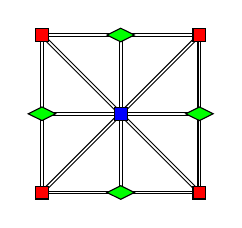
\begin{tikzpicture}
\draw (-1, -1)--(1, -1) [mir];
\draw (-1, 0)--(1, 0) [mir];
\draw (-1, 1)--(1, 1) [mir];

\draw (-1, -1)--(-1, 1) [mir];
\draw (0, -1)--(0, 1) [mir];
\draw (1, -1)--(1, 1) [mir];

\draw (-1, -1)--(1, 1) [mir];
\draw (-1, 1)--(1, -1) [mir];

\draw (0, 0) node [d4, fill=blue] {};

\draw (-1, 0) node [d2, fill=green] {};
\draw (1, 0) node [d2, fill=green] {};
\draw (0, 1) node [d2, fill=green] {};
\draw (0, -1) node [d2, fill=green] {};

\draw (-1, -1) node [d4, fill=red] {};
\draw (-1, 1) node [d4, fill=red] {};
\draw (1, -1) node [d4, fill=red] {};
\draw (1, 1) node [d4, fill=red] {};

\end{tikzpicture}
\end{document}
